\documentclass[10pt]{report}
\title{\textbf{PostOffice Specification v0.1}}
\author{Dillon Dixon}
\date{August 30, 2013}
\usepackage{graphicx}
\usepackage{geometry}
\usepackage{float}
\usepackage{CJK}

\usepackage{tikz}

\usetikzlibrary{arrows,shadows}
\usepackage{pgf-umlsd}

\geometry{a4paper,tmargin=1.5cm, bmargin=1.5cm, lmargin=2cm, rmargin=2.5cm, headheight=3em, headsep=1.5cm, footskip=1cm} 
\usepackage[parfill]{parskip}
\begin{document}

\maketitle
\tableofcontents

\chapter{Introduction}

PostOffice is a library designed for interprocess communication via sockets to a \emph{Post Office} server daemon. Clients register a password protected \emph{mailbox} with the server daemon, which can be used to send and receive mail to and from other client mailboxes.

There are many existing message passing solutions, such as \emph{DBus}\footnote{http://dbus.freedesktop.org} and \emph{CORBA}\footnote{http://www.corba.org/}, but most are highly generalized and intended for large scale deployment, often resulting in hefty documentation and buggy language bindings.

\emph{PostOffice} was created in response to those developers who want a simple, platform independent and intuitive way for passing messages between processes. The whole system uses the common terminology of the actual physical mail system, making it immediately familiar.

This document functions as a description of the underlying protocol for those interested in implementing a \emph{Client} binding for a different programming language.

\chapter{Architecture}

\section{Overview}

\emph{PostOffice} functions, as defined by its name, like a post office. An abstract description of the functionality can be found in figure \ref{fig:post_office} below.

\begin{figure}[H]
\centering
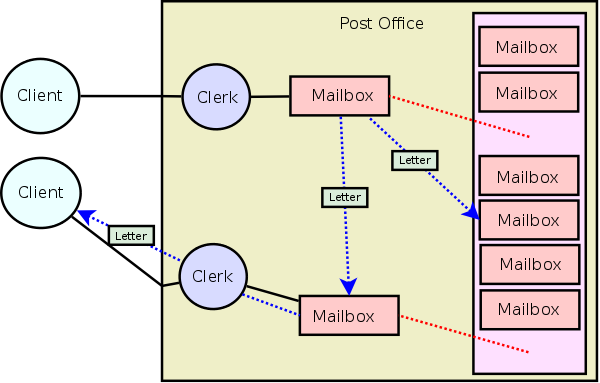
\includegraphics[scale=0.4]{postoffice_spec.png}
\caption{Abstract Diagram of Post Office}
\label{fig:post_office}
\end{figure}

Clients connect to a \emph{Clerk} (a thread on the server to handle the particular client connection). Clerks perform commands server side on behalf of the client, which involve sending and receiving mail, among other operations. When a client connects to a clerk, they must bind to a particular mailbox. If one does not exist, the clerk can create one for them. Clerks can also destroy them when they are no longer needed. Clients can create and destroy as many mailboxes as they like.

\emph{Mailboxes} are the identifiers for clients in the post office. All mailboxes have unique identifiers. Like a physical mailbox, a mailbox can receive and store messages for a particular client while they are disconnected. A mailbox may be checked out by only a single clerk at a time.

Once a mailbox is checked out, a client can send and receive messages via the clerk. Any outgoing mail will be recorded as having originated at that particular mailbox. Mailboxes are password protected to allow only their creators to use them. The protocol by which actions are performed through the client is documented in later sections.

\section{Control Flags}

The following control flag enumerations are used for communication between the client connector and the post office server. Each code is represented by a single byte when sent over the socket.

The following list of flags in table \ref{fig:req_table} are commands that the client can make to the server to request actions.

\begin{table}[h]
	\centering
	\caption{Client requests to the server}
	\begin{tabular}{|l|c|p{11cm}|}
		\hline\multicolumn{1}{|c|}{\bfseries Name} & \multicolumn{1}{|c|}{\bfseries Code} & \multicolumn{1}{|c|}{\bfseries Description} \\ \hline
		REQBOX & 0 & \emph{Request box} -- Checkout an existing mailbox.\\ \hline
		RETBOX & 1 & \emph{Return box} -- Return an existing mailbox.\\ \hline
		CREATEBOX & 2 & Create a new mailbox.\\ \hline
		REMOVEBOX & 3 & Delete/destroy an existing mailbox.\\ \hline
		SENDLETTER & 4 & Send a letter to a mailbox.\\ \hline
		GETMAIL & 5 & Retrieve mail from the connected mailbox.\\ \hline
		NEXTLETTER* & 6 & Request the next letter in the connected mailbox.\\ \hline
		SATIATED* & 7 & Request for no further message transfers from the connected mailbox.\\ \hline
		EMPTYBOX & 8 & Empty the connected mailbox.\\ \hline
		DISCONNECT & 9 & Indicate a disconnect from the post office server (impeding socket closure).\\ \hline
	\end{tabular}
	\label{fig:req_table}
\end{table}

Request flags marked by an asterisk (*) are \emph{non-initiating} flags, meaning they cannot be used as immediate requests to a server, and only as part of another request.

The following list of flags in table \ref{fig:resp_table} are responses the server can make to client requests.

\begin{table}[h]
	\centering
	\caption{Client requests to the server}
	\begin{tabular}{|l|c|p{12cm}|}
		\hline\multicolumn{1}{|c|}{\bfseries Name} & \multicolumn{1}{|c|}{\bfseries Code} & \multicolumn{1}{|c|}{\bfseries Description} \\ \hline
		Name & Code & Description\\ \hline
		REQGRANTED & 0 & \emph{Request granted} -- Indicates the successful completion of a request.\\ \hline
		REQDATA & 1 & \emph{Request data} -- Indicates the client should now send some data.\\ \hline
		NOAUTH & 2 & Made a request which the client is not authorized to perform.\\ \hline
		BADCOMMAND & 3 & Received an unknown command code from the client (possible sync issues).\\ \hline
		ALREADYCONN & 4 & The client is already connected to a mailbox.\\ \hline
		MAILTIMEOUT & 5 & The waiting period for new mail has expired.\\ \hline
		BOXEXISTS & 6 & A box was requested to be created, but it already exists.\\ \hline
		NONEXISTBOX & 7 & A request was made on a box that does not exist.\\ \hline
		NOBOXCONN & 8 & A request was made on a mailbox, but no mailbox connection exists.\\ \hline
		BOXINUSE & 9 & A request has been made with a mailbox that has been checked out by another client.\\ \hline
		DELFAIL & 10 & Failed to deliver a message (the recipient does not exist).\\ \hline
		SHUTDOWN & 11 & The server is shutting down and will be closing all sockets.\\ \hline
		COMMTIMEOUT & 12 & The client's response time has expired; server is going to disconnect.\\ \hline
		NOMAIL & 13 & There is no mail in the mailbox.\\ \hline
		INMAIL & 14 & There is mail in the mailbox.\\ \hline
	\end{tabular}
	\label{fig:resp_table}
\end{table}

\section{Data Restrictions}

\subsection{Identifiers}

Identifiers specified by clients must only be those recognizable by the following regular expression: \verb|([^,\.]+\.)*[^,\.]+|

These include expressions of the form: canada.government.primeminister, america.government.president... and so on. It is similar to the \emph{Java package naming hierarchy}\footnote{http://docs.oracle.com/javase/tutorial/java/package/namingpkgs.html}.

The only disallowed character in an identifier is the comma (0x2C), as it is used to separate identifiers in a list. This leaves support for all international characters, allowing for very localized identifiers such as: \begin{CJK*}{UTF8}{min}
中國.政府.首腦.\end{CJK*}

\subsection{Passwords}

All passwords must be 16-byte (128-bit) MD5-hashes. This is the only hashing type that the server supports.

\section{Variable Length Data Transmission}

Some of the data transferred between the server and the client is ambiguous in length (i.e. mailbox identifiers, messages. etc). Two different schemes are used for handling this.

\subsection{String data}
\label{string_data}

For string data (i.e. identifiers), the data is sent in a \emph{modified} UTF-8 format that looks as follows: \verb|<2-bytes><UTF-8 String bytes>|. The initial 2-bytes are a short integer storing the length of the following UTF-8 string. This limits all identifiers to a maximum length of 8,192 characters. In all sequence diagrams, data of this type will be marked with \emph{\textbf{S}}.

\subsection{Binary data}
\label{bin_data}

For binary data (i.e. message payloads), the data is sent in a similar way to string data as follows: \verb|<4-bytes><UTF-8 Data bytes>|. The initial 4-bytes are an integer storing the length of the binary stream. This limits all message payloads to a length of 4294967296 bits, or 512 megabytes. In all sequence diagrams, data of this type will be marked with \emph{\textbf{B}}.

\chapter{Action Sequences}

\section{Introduction}

The section defines the protocol by which a client's language binding \emph{connector} and the server communicate. All the diagrams are presented as \emph{sequence diagrams}\footnote{http://en.wikipedia.org/wiki/Sequence\_diagram} to show how data is sent and synchronization between client and server is maintained.

\section{Creating a mailbox}

Clients must \emph{checkout} a mailbox before they can begin sending or receiving messages. For new clients connecting to the server, a mailbox they can connect to may not already exist. The following sequence diagram  in figure \ref{seq_create} below explains this process.

\begin{figure}[H]
\centering
	\begin{sequencediagram}
	
		\newthread[0]{u}{Client}
		\newthread[7]{b}{Post Office Server}
		
		\begin{call}{u}{REQ.CREATEBOX}{b}{RESP.REQDATA}\end{call}
		\begin{call}{u}{\emph{identifier} [\emph{\textbf{S}}]}{b}{RESP.REQDATA}\end{call}
		
		\begin{call}{u}{\emph{password hash} [\emph{\textbf{16-bytes}}]}{b}{\shortstack{\textbf{[\underline{IF} the mailbox already exists]} RESP.BOXEXISTS \\ \textbf{[\underline{ELSE} create the mailbox]} RESP.REQ}} \postlevel \end{call}
		
	\end{sequencediagram}
	\caption{Protocol for creating a mailbox.}
	\label{seq_create}
\end{figure}

\newpage

\section{Requesting a mailbox}

After a client has created a mailbox, they can \emph{check it out} to begin sending and receiving messages. The following sequence diagram in figure \ref{seq_checkout} below explains this process.

\begin{figure}[H]
\centering
	\begin{sequencediagram}
	
		\newthread[0]{u}{Client}
		\newthread[10]{b}{Post Office Server}
		
		\begin{sdblock}{IF}{The clerk is already connected to a mailbox.}
			\begin{call}{u}{REQ.REQBOX}{b}{RESP.ALREADYCONN}
			\end{call}
		\end{sdblock}
		
		\begin{sdblock}{ELSE}{Request details for checkout.}
		\begin{call}{u}{REQ.REQBOX}{b}{RESP.REQDATA}\end{call}
		\begin{call}{u}{\emph{identifier} [\emph{\textbf{S}}]}{b}{RESP.REQDATA}\end{call}
			
		\begin{call}{u}{\emph{password hash} [\emph{\textbf{16-bytes}}]}{b}{\shortstack{\textbf{[\underline{IF} the credentials are incorrect]} RESP.NOAUTH \\ \textbf{[\underline{ELSE IF} the mailbox is already in use]} RESP.BOXINUSE \\ \textbf{[\underline{ELSE IF} the mailbox does not exist]} RESP.NONEXISTMAILBOX \\ \textbf{[\underline{ELSE} checkout the mailbox]} RESP.REQGRANTED}} \postlevel \postlevel \postlevel\end{call}
		
		\end{sdblock}
		
	\end{sequencediagram}
	\caption{Protocol for requesting a mailbox.}
	\label{seq_checkout}
\end{figure}

\section{Returning a mailbox}

After a client has checked out a mailbox and completed using it, they must \emph{return} the mailbox before checking out another one.

\begin{figure}[H]
\centering
	\begin{sequencediagram}
	
		\newthread[0]{u}{Client}
		\newthread[10]{b}{Post Office Server}
		
		\begin{call}{u}{REQ.RETBOX}{b}{\shortstack{\textbf{[\underline{IF} there is no existing mailbox connection]} RESP.NOBOXCONN \\ \textbf{[\underline{ELSE} return the mailbox]} RESP.REQGRANTED}} \postlevel\end{call}
		
	\end{sequencediagram}
	\caption{Protocol for returning a mailbox.}
	\label{seq_checkout}
\end{figure}

Keep in mind, a \underline{reliable} implementation of the \emph{PostOffice} server should automatically return mailboxes should the client randomly disconnect and the socket terminate. It is always good practice to disconnect properly though, rather than causing an exception in the clerk thread on the server. 

\section{Removing a mailbox}

In the event of a client disconnecting from the \emph{PostOffice} server, the client may find it desirable to completely remove the mailbox as to not give other sending clients the impression that they are still actively accepting messsages. As long as a client is \underline{presently connected} to a mailbox, they can destroy it. This process is documented in figure \ref{seq_remove} below.

\begin{figure}[H]
\centering
	\begin{sequencediagram}
	
		\newthread[0]{u}{Client}
		\newthread[10]{b}{Post Office Server}
		
		\begin{sdblock}{IF}{The clerk is not already connected to a mailbox.}
			\begin{call}{u}{REQ.REMOVEBOX}{b}{RESP.NOBOXCONN}
			\end{call}
		\end{sdblock}
		
		\begin{sdblock}{ELSE}{Request details for checkout.}
		\begin{call}{u}{REQ.REMOVEBOX}{b}{\shortstack{\textbf{[\underline{IF} the credentials are incorrect]} RESP.NOAUTH \\ \textbf{[\underline{ELSE IF} the mailbox does not exist]} RESP.NONEXISTMAILBOX \\ \textbf{[\underline{ELSE} remove the mailbox]} RESP.REQGRANTED}} \postlevel \postlevel \end{call}
		
		\end{sdblock}
		
	\end{sequencediagram}
	\caption{Protocol for removing a mailbox.}
	\label{seq_remove}
\end{figure}

\section{Emptying a mailbox}

Sometimes a client may find it desirable to completely flush all the messages from the mailbox before waiting on a new one, as to ensure any messages they receive are relatively new. This process is documented in figure \ref{seq_empty} below.

\begin{figure}[H]
\centering
	\begin{sequencediagram}
	
		\newthread[0]{u}{Client}
		\newthread[10]{b}{Post Office Server}
		
		\begin{call}{u}{REQ.EMPTYBOX}{b}{\shortstack{\textbf{[\underline{IF} the user has not connected to a mailbox]} RESP.NOBOXCONN \\ \textbf{[\underline{ELSE} empty the mailbox]} RESP.REQGRANTED}} \postlevel \end{call}
		
	\end{sequencediagram}
	\caption{Protocol for emptying a mailbox.}
	\label{seq_empty}
\end{figure}

\newpage

\section{Sending a message}

Clients can send a message to an unlimited number of recipients. This process is documented in figure \ref{seq_sendmes} below.

\begin{figure}[H]
\centering
	\begin{sequencediagram}
	
		\newthread[0]{u}{Client}
		\newthread[10]{b}{Post Office Server}
		
		\begin{sdblock}{IF}{The clerk is not connected to a mailbox.}
			\begin{call}{u}{REQ.REQBOX}{b}{RESP.NOBOXCONN}
			\end{call}
		\end{sdblock}
		
		\begin{sdblock}{ELSE}{Continue with sending the message.}
		\begin{call}{u}{REQ.REQBOX}{b}{RESP.REQDATA}\end{call}
		
		\begin{call}{u}{\emph{Number of incoming recipients} [\emph{\textbf{4-bytes}}] + \emph{identifiers}  (consecutive [\emph{\textbf{S}}])}{b}{RESP.REQDATA}\end{call}
		
		\begin{call}{u}{\emph{message} [\emph{\textbf{B}}]}{b}{\shortstack{\textbf{[\underline{IF} delivery fails to some recipients]} RESP.DELFAIL \\ + \emph{Number of non-existent recipients} [\emph{\textbf{4-bytes}}] \\ + \emph{identifiers} (consecutive [\emph{\textbf{S}}]) \\ \textbf{[\underline{ELSE} report success]} RESP.REQGRANTED}} \postlevel \postlevel \postlevel \end{call}
		
		\end{sdblock}
		
	\end{sequencediagram}
	\caption{Protocol for sending a message.}
	\label{seq_sendmes}
\end{figure}

Recipients are specified first by a 4-byte integer indicating the number of recipients, followed by all the identifiers in the modified UTF-8 format described in section \ref{string_data}. This format is also used for sending back the list of non-existent recipients to the client, should a delivery failure occur.

\newpage

\section{Receiving messages}

Clients receive messages in the order they were received in the mailbox. If the client was looking for a specific message, and it is behind several others, then the client must download those messages first before getting to the desired one. 


\begin{figure}[H]
\centering
	\begin{sequencediagram}
	
		\newthread[0]{u}{Client}
		\newthread[10]{b}{Post Office Server}
		
		\begin{sdblock}{IF}{The clerk is not connected to a mailbox.}
			\begin{call}{u}{REQ.REQBOX}{b}{RESP.NOBOXCONN}
			\end{call}
		\end{sdblock}
		
		\begin{sdblock}{ELSE}{Continue with receiving messages.}
		\begin{call}{u}{REQ.REQBOX}{b}{RESP.REQDATA}\end{call}
		
		
		\begin{sdblock}{LOOP}{}
			\begin{sdblock}{IF}{There is no mail and no timeout given (equal to 0). \underline{\textbf{TERMINATE LOOP}}}
				\begin{call}{u}{\emph{timeout in milliseconds} [\emph{\textbf{4-bytes}}]}{b}{RESP.MAILTIMEOUT}
				\end{call}
			\end{sdblock}
		
			\begin{sdblock}{ELSE}{If a timeout has been specified, or there is mail.}
				\begin{call}{u}{\emph{timeout in milliseconds} [\emph{\textbf{4-bytes}}]}{b}{RESP.REQDATA}
				\end{call}
			
				\begin{sdblock}{IF}{The client wants the next available letter.}
					
					\begin{call}{u}{REQ.NEXTLETTER}{b}{\shortstack{\textbf{[\underline{IF} mail available + \textbf{\underline{LOOP}}]} RESP.INMAIL + \emph{identifier} + message [\emph{\textbf{B}}] \\ \textbf{[\underline{ELSE} timeout waiting]} RESP.MAILTIMEOUT}} \postlevel \end{call}
				\end{sdblock}
		
				\begin{sdblock}{ELSE}{The client does not want anymore mail.}
					\begin{call}{u}{REQ.SATIATED}{b}{RESP.REQGRANTED}
					\end{call}
				\end{sdblock}
			
			\end{sdblock}
		\end{sdblock}
		
		\end{sdblock}
		
	\end{sequencediagram}
	\caption{Protocol for sending a message.}
	\label{seq_sendmes}
\end{figure}

Receiving mail is the most complicated process the client must perform. When the client requests mail, it must send the server a ``timeout''. This is the amount of time the client would like to wait around for a message to show up before relenting to the fact that there is no mail (in milliseconds).

If there is no mail, but the client has specified a timeout, the server will block the client until the timeout has expired. If a message arrives before the timeout expires, the message will be forwarded to the client. If the client is not satisfied with that message, it can respond with \emph{REQ.NEXTLETTER} to continue waiting for more messages until the timer expires. If the client is satisfied, it can respond with \emph{REQ.SATISFIED}. This will tell the server to stop waiting for new mail.

If the client does not specify a timeout, and there is no mail, then the server will immediately notify the client that it has timed out waiting. Otherwise, the same process as above occurs.

If the server times out \emph{while there is mail available}, then it will \underline{NOT} send the \emph{RESP.MAILTIMEOUT} response. This allows the client to receive as many of the messages in the mailbox as it would like until it is satisfied.

A \emph{good} server implementation should \underline{NOT} remove messages from the queue until the client has confirmed receipt with either a \emph{REQ.NEXTLETTER} or \emph{REQ.SATISFIED}. This prevents data loss.
\end{document}